% !TeX program = xelatex
% COSTTRACE research manuscript draft
% This manuscript skeleton is evidence-based and uses only metrics/artifacts
% present in the repository as of 2026-06-24.

\documentclass[11pt,a4paper]{article}

\usepackage[a4paper,margin=1in]{geometry}
\usepackage{iftex}
\ifPDFTeX
  \usepackage[T1]{fontenc}
  \usepackage[utf8]{inputenc}
  \usepackage{newtxtext,newtxmath}
\else
  \usepackage{fontspec}
  \setmainfont{Times New Roman}
  \setsansfont{Arial}
  \setmonofont{Consolas}
\fi

\usepackage{setspace}
\doublespacing
\usepackage{microtype}
\usepackage{amsmath,amssymb}
\usepackage{graphicx}
\usepackage{booktabs}
\usepackage{array}
\usepackage{tabularx}
\usepackage{longtable}
\usepackage{caption}
\usepackage{subcaption}
\usepackage[numbers,sort&compress]{natbib}
\usepackage{hyperref}
\usepackage{xcolor}

\hypersetup{
  colorlinks=true,
  linkcolor=black,
  citecolor=blue,
  urlcolor=blue,
  pdftitle={Budget-Constrained Node Intervention in Household Epidemic Contact Networks Using Graph Learning},
  pdfauthor={TODO: Authors},
  pdfkeywords={contact network, graph learning, epidemic intervention, GraphSAGE, SARS-CoV-2}
}

\graphicspath{
  {../visualizations/}
  {../results/figures/topology/}
  {../results/figures/intervention/}
  {../results/gephi/}
  {visualizations/}
  {results/figures/topology/}
  {results/figures/intervention/}
  {results/gephi/}
}

\newcommand{\TODO}[1]{\textcolor{red}{[TODO: #1]}}
\newcommand{\costtrace}{\textsc{CostTrace}}

\title{Budget-Constrained Node Intervention in Household Epidemic Contact Networks Using Graph Learning}

\author{
  TODO: Author 1\thanks{TODO: Corresponding author email, phone, ORCID if available.}\\
  TODO: Affiliation 1
  \and
  TODO: Author 2\\
  TODO: Affiliation 2
  \and
  TODO: Author 3\\
  TODO: Affiliation 3
  \and
  TODO: Author 4\\
  TODO: Affiliation 4
}

\date{}

\begin{document}
\maketitle

\begin{abstract}
Household contact networks provide a structured representation of close physical interactions that may shape infectious disease transmission. This study presents \costtrace, a reproducible pipeline for budget-constrained node intervention in an empirical SARS-CoV-2 household contact network. Using the SASHTS dataset, we aggregate 140,542 raw proximity events into a weighted undirected graph of 340 individuals, 542 contact edges, and 88 household components. The pipeline computes topology, centrality, Louvain communities, interpretable composite risk scores, and a lightweight pure-PyTorch Weighted GraphSAGE proxy for node-level infection-risk ranking. We compare Random, Degree, Betweenness, and GraphSAGE-based strategies under 1\%, 5\%, and 10\% intervention budgets using counterfactual transmission blocking and household-level SIR simulation. The household graph is globally sparse but locally dense, with average household density 0.9633 and Louvain modularity 0.9696 with 100\% household agreement. The GraphSAGE proxy achieves test AUC 0.7669 and average precision 0.8995. Under counterfactual evaluation, Degree performs best at the 1\% budget with a 4.6\% prevention rate, while GraphSAGE performs best at 5\% and 10\%, reaching 26.8\% and 49.0\% prevention rates and SIR reductions of 22.2\% and 42.7\%, respectively. These findings suggest that simple centrality can be competitive under extremely scarce budgets, whereas learned multi-feature ranking becomes more useful when intervention capacity increases. The study is a proof of concept on one household dataset and should not be interpreted as a clinical decision system without further validation.
\end{abstract}

\noindent\textbf{Keywords:} contact network; epidemic intervention; budget-constrained node selection; GraphSAGE; social network analysis; SARS-CoV-2; SIR simulation.

\section*{TODO Before Submission}

\begin{itemize}
  \item Confirm the exact target journal, article type, and reference style.
  \item Fill final author names, affiliations, emails, corresponding author, phone, and ORCID.
  \item Confirm whether a Vietnamese title page and Vietnamese abstract are required.
  \item Replace all provisional wording if Phase 04--05 upgrades produce new validated results.
  \item Confirm raw-data redistribution permissions; otherwise cite data source only and omit raw data from public release.
\end{itemize}

\section{Introduction}

Infectious disease spread depends not only on individual-level susceptibility but also on the structure of physical contact. Classical compartmental models such as SIR assume population-level mixing, whereas empirical contact networks represent individuals as nodes and physical interactions as edges. In this representation, degree captures direct exposure opportunity, weighted degree captures cumulative interaction intensity, betweenness captures bridging structure, and household communities can define local transmission environments.

Digital and sensor-based contact data create a practical decision problem after risk estimation: public-health resources are limited, and only a subset of individuals can be prioritized for testing, monitoring, isolation, or follow-up. This motivates a budget-constrained node selection problem: given a contact graph and a limited intervention budget, which nodes should be selected to reduce transmission most effectively?

\costtrace\ addresses this question using the SASHTS household transmission dataset. The project converts proximity sensor events into a weighted contact graph, characterizes household topology, estimates node risk with interpretable centrality features and a Weighted GraphSAGE proxy, and evaluates top-\(k\) intervention strategies under fixed budgets. Unlike source-tracing methods such as DeepTrace, this work does not claim to infer the original infection source. Instead, it focuses on downstream intervention ranking under constrained resources.

This manuscript asks three research questions:

\begin{enumerate}
  \item How does the structure of the SASHTS household contact network shape the interpretation of centrality, community structure, and intervention ranking?
  \item Under fixed 1\%, 5\%, and 10\% node-selection budgets, how do Random, Degree, Betweenness, and GraphSAGE-based ranking strategies compare in counterfactual transmission blocking?
  \item Do the same strategies show consistent effects under household-level SIR simulation, and how should recommendations change with available intervention capacity?
\end{enumerate}

The main contributions are: (i) a reproducible pipeline for weighted household contact graph construction and analysis; (ii) a comparison of classical network heuristics and a graph-learning risk score for budget-constrained intervention; and (iii) dual evaluation through observed-edge counterfactual analysis and stochastic SIR simulation.

\section{Related Work}

\TODO{Phase 02 should replace this section with a full related-work synthesis and verified citation base. Do not submit with this placeholder section.}

Contact tracing, epidemic network modeling, influence maximization, vaccination strategies, and graph neural networks form the relevant literature base for this study. GraphSAGE provides an inductive graph representation learning framework \cite{hamilton2017graphsage}. Community detection with Louvain is commonly used to identify densely connected modules in weighted networks \cite{blondel2008louvain}. Epidemic dynamics on networks are grounded in the theory of network-based infectious disease models \cite{kiss2017epidemics,keeling2005networks}. The present work uses these tools for a constrained intervention-ranking task on an empirical household contact network.

\section{Materials and Methods}

\subsection{Dataset}

The study uses the SASHTS -- South Africa Household Transmission Study -- proximity sensor and epidemiological dataset. Repository evidence records 140,542 raw proximity events, 340 individuals, 88 households, and 542 aggregated weighted contact edges after preprocessing. The dataset includes site labels, SARS status, index/contact role, age group, sex, susceptibility, household identifiers, and selected household exposure indicators.

The current repository note reports that Soweto records include real timestamps for the collection period 2020-11-18 to 2021-08-19, whereas Klerksdorp records do not contain real timestamps. Therefore, the current analysis is treated primarily as a static weighted household contact graph rather than as a fully temporal intervention model.

\begin{table}[htbp]
\centering
\caption{Dataset and graph summary. Values are read from repository artifacts under \texttt{data/processed/eda\_summary.json} and \texttt{results/metrics/basic\_metrics.json}.}
\label{tab:dataset-summary}
\begin{tabular}{lr}
\toprule
Quantity & Value \\
\midrule
Raw proximity events & 140,542 \\
Individuals / nodes & 340 \\
Aggregated weighted contact edges & 542 \\
Household components & 88 \\
Average household size & 3.86 \\
Average household density & 0.9633 \\
Average household diameter & 1.17 \\
Average household clustering & 0.7994 \\
SARS positive individuals & 241 \\
SARS negative individuals & 99 \\
Observed attack rate & 70.9\% \\
\bottomrule
\end{tabular}
\end{table}

\subsection{Preprocessing and Graph Construction}

Raw event records are curated by removing self-loops, canonicalizing unordered dyads so that A--B and B--A are treated as the same contact pair, and aggregating repeated proximity events into pair-level weighted edges. The edge weight is the total contact duration in seconds, and the number of raw contact events is retained as a contact-frequency attribute. Each participant is represented as a node, and metadata are attached as node attributes.

The graph is undirected and weighted:
\[
G = (V, E, W),
\]
where \(V\) is the set of individuals, \(E\) is the set of aggregated contact pairs, and \(W\) stores total contact duration.

\subsection{Topology, Centrality, and Community Detection}

The graph is analyzed as 88 connected household components. This is necessary because the global graph is disconnected by construction and does not contain cross-household edges. For each node, the pipeline computes degree centrality, weighted degree, betweenness centrality, and closeness centrality. Louvain community detection is applied using total contact duration as edge weight.

An interpretable composite risk score is computed as:

\[
\mathrm{risk}(v) =
0.35\,d_v +
0.30\,w_v +
0.20\,b_v +
0.15\,s_v ,
\]

where \(d_v\) is normalized degree centrality, \(w_v\) is normalized weighted degree, \(b_v\) is normalized betweenness centrality, and \(s_v\) encodes whether the participant slept in the same room as the index case.

\subsection{Weighted GraphSAGE Proxy}

The graph-learning model is a lightweight pure-PyTorch Weighted GraphSAGE classifier. It uses 11 input features: normalized degree centrality, normalized weighted degree, normalized betweenness centrality, normalized closeness centrality, sleep-room exposure, caregiving exposure, scaled age group, sex, susceptibility, site, and index-case role.

Edge weights are transformed as \(\log(1 + \mathrm{duration})\) and row-normalized for weighted mean aggregation. The model is trained with a stratified 70\%/15\%/15\% train/validation/test split, 500 epochs, Adam optimization, learning rate 0.01, weight decay \(5\times 10^{-4}\), and seed 42. The output probability is used as a ranking score for top-\(k\) selection.

\TODO{Phase 03 and Phase 04 should revisit split protocol and leakage risk. Current node-level stratified splitting may overestimate generalization because household components can be shared across splits.}

\subsection{Budget-Constrained Intervention Strategies}

Four strategies are evaluated at 1\%, 5\%, and 10\% budgets:

\begin{itemize}
  \item Random: uniformly random node selection, averaged over repeated samples.
  \item Degree: select nodes with highest degree centrality.
  \item Betweenness: select nodes with highest betweenness centrality.
  \item GraphSAGE: select nodes with highest predicted infection probability.
\end{itemize}

The selected budgets correspond to 3, 17, and 34 selected nodes, respectively.

\subsection{Counterfactual Transmission Evaluation}

Counterfactual evaluation estimates how many observed transmission edges and SARS-positive contact cases would be blocked if selected nodes were successfully intervened on. This analysis is not a causal claim about real-world deployment; it is an observed-edge blocking analysis under a node-removal assumption.

The prevention rate is:
\[
\mathrm{PreventionRate} =
\frac{\left|\mathrm{PreventedSecondaryCases}\right|}
{\left|\mathrm{SARSPositiveContacts}\right|}
\times 100.
\]

\subsection{SIR Simulation}

The SIR evaluation is run per household component with one index case as seed. The repository configuration uses infection rate \(\beta=0.25\), recovery rate \(\gamma=0.10\), horizon \(T=30\) days, 50 Monte Carlo runs, and seed 42. Edge transmission probability is scaled by log contact duration. The baseline mean infected per household is 3.4214.

\TODO{Phase 05 should add sensitivity analysis over beta, gamma, time horizon, and Monte Carlo runs before final submission.}

\section{Results}

\subsection{Network Structure}

The SASHTS graph contains 340 nodes and 542 weighted edges across 88 connected household components. The global network is sparse, but household subgraphs are dense: average household density is 0.9633. Louvain community detection identifies 88 communities with modularity 0.9696 and 100\% agreement with household labels, indicating that household boundaries dominate the observed network structure.

\begin{figure}[htbp]
\centering
\includegraphics[width=0.92\textwidth]{network_overview.png}
\caption{Contact network overview. Node size reflects degree centrality, colors indicate household/community structure, and high-risk nodes are highlighted. Source artifact: \texttt{visualizations/network\_overview.png}.}
\label{fig:network-overview}
\end{figure}

\subsection{GraphSAGE Risk Model}

The Weighted GraphSAGE proxy achieves test AUC 0.7669 and test average precision 0.8995. The large train-test gap suggests overfitting risk, but the average precision indicates that the model can still provide a useful ranking signal for top-\(k\) prioritization in this proof-of-concept setting.

\begin{table}[htbp]
\centering
\caption{Weighted GraphSAGE performance. Values are read from \texttt{results/model/gnn\_metrics.json}.}
\label{tab:gnn-performance}
\begin{tabular}{lrrrrr}
\toprule
Split & AUC & AP & F1 & Precision & Recall \\
\midrule
Train & 0.9914 & 0.9966 & 0.9619 & 0.9480 & 0.9762 \\
Validation & 0.8036 & 0.9162 & 0.8732 & 0.8857 & 0.8611 \\
Test & 0.7669 & 0.8995 & 0.8158 & 0.7949 & 0.8378 \\
\bottomrule
\end{tabular}
\end{table}

\subsection{Intervention Performance}

Table~\ref{tab:final-comparison} summarizes the final intervention comparison. At the 1\% budget, Degree achieves the highest counterfactual prevention rate, 4.6\%. At 5\% and 10\%, GraphSAGE is the strongest strategy, achieving prevention rates of 26.8\% and 49.0\%, and SIR reductions of 22.2\% and 42.7\%.

\begin{table}[htbp]
\centering
\caption{Final intervention comparison by budget and strategy. Values are read from \texttt{results/intervention/final\_comparison.csv}.}
\label{tab:final-comparison}
\begin{tabular}{rrlrrrr}
\toprule
Budget & Nodes & Strategy & Precision@k & Transmission coverage & Prevention rate & SIR reduction \\
\midrule
1\% & 3 & Degree & 100.0 & 2.4 & 4.6 & 2.0 \\
1\% & 3 & GraphSAGE & 100.0 & 2.1 & 3.9 & 3.8 \\
1\% & 3 & Random & 71.7 & 1.7 & 3.3 & 1.2 \\
1\% & 3 & Betweenness & 66.7 & 0.3 & 0.7 & 1.0 \\
5\% & 17 & GraphSAGE & 100.0 & 14.3 & 26.8 & 22.2 \\
5\% & 17 & Random & 70.8 & 9.7 & 17.4 & 7.6 \\
5\% & 17 & Betweenness & 64.7 & 6.3 & 11.8 & 8.9 \\
5\% & 17 & Degree & 64.7 & 8.4 & 10.5 & 6.6 \\
10\% & 34 & GraphSAGE & 100.0 & 26.2 & 49.0 & 42.7 \\
10\% & 34 & Random & 70.7 & 19.2 & 33.0 & 16.8 \\
10\% & 34 & Betweenness & 70.6 & 16.4 & 30.7 & 20.4 \\
10\% & 34 & Degree & 64.7 & 17.1 & 22.2 & 14.6 \\
\bottomrule
\end{tabular}
\end{table}

\begin{figure}[htbp]
\centering
\begin{subfigure}{0.48\textwidth}
  \centering
  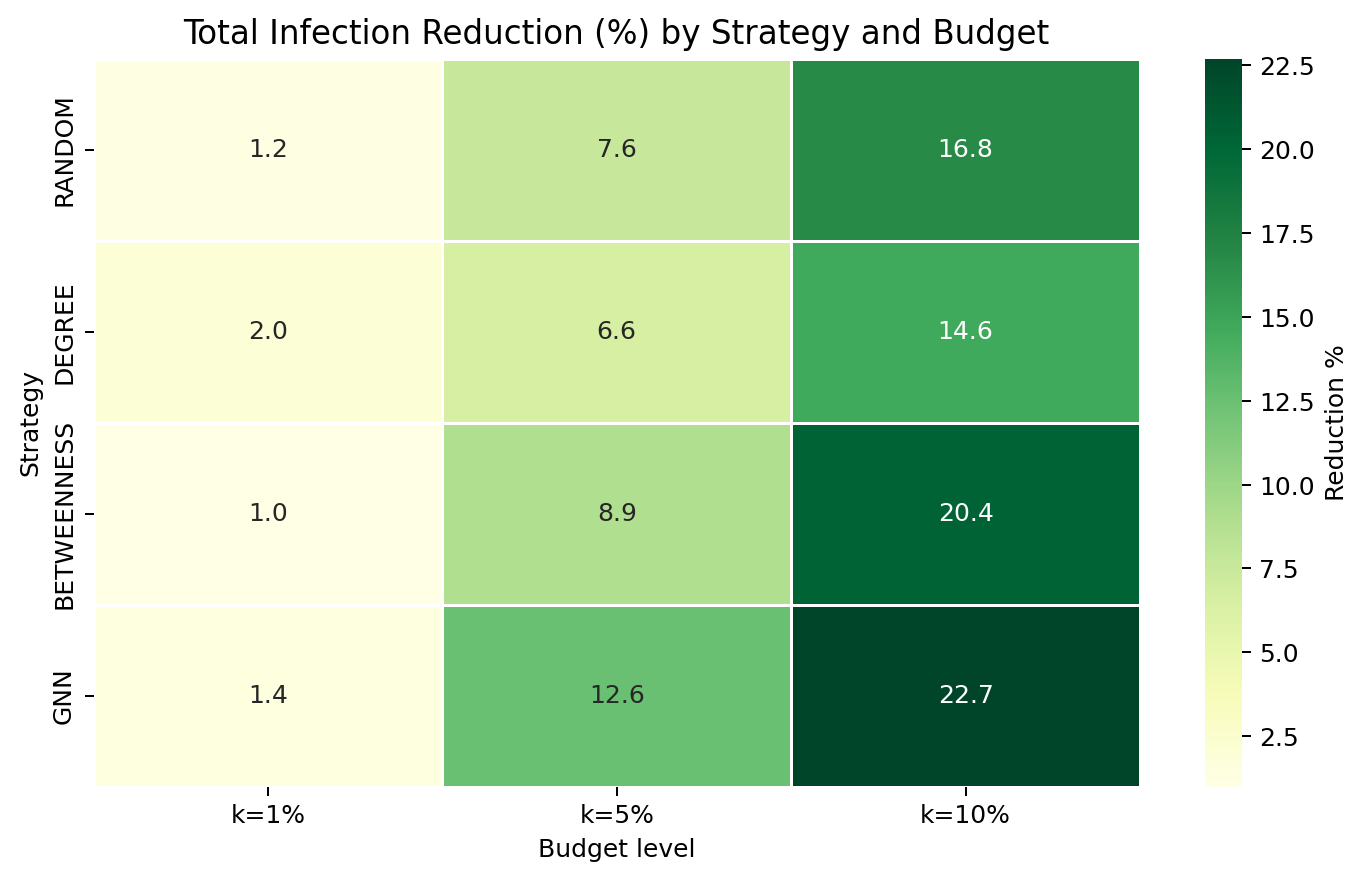
\includegraphics[width=\textwidth]{chart_heatmap.png}
  \caption{Counterfactual prevention rate.}
\end{subfigure}
\hfill
\begin{subfigure}{0.48\textwidth}
  \centering
  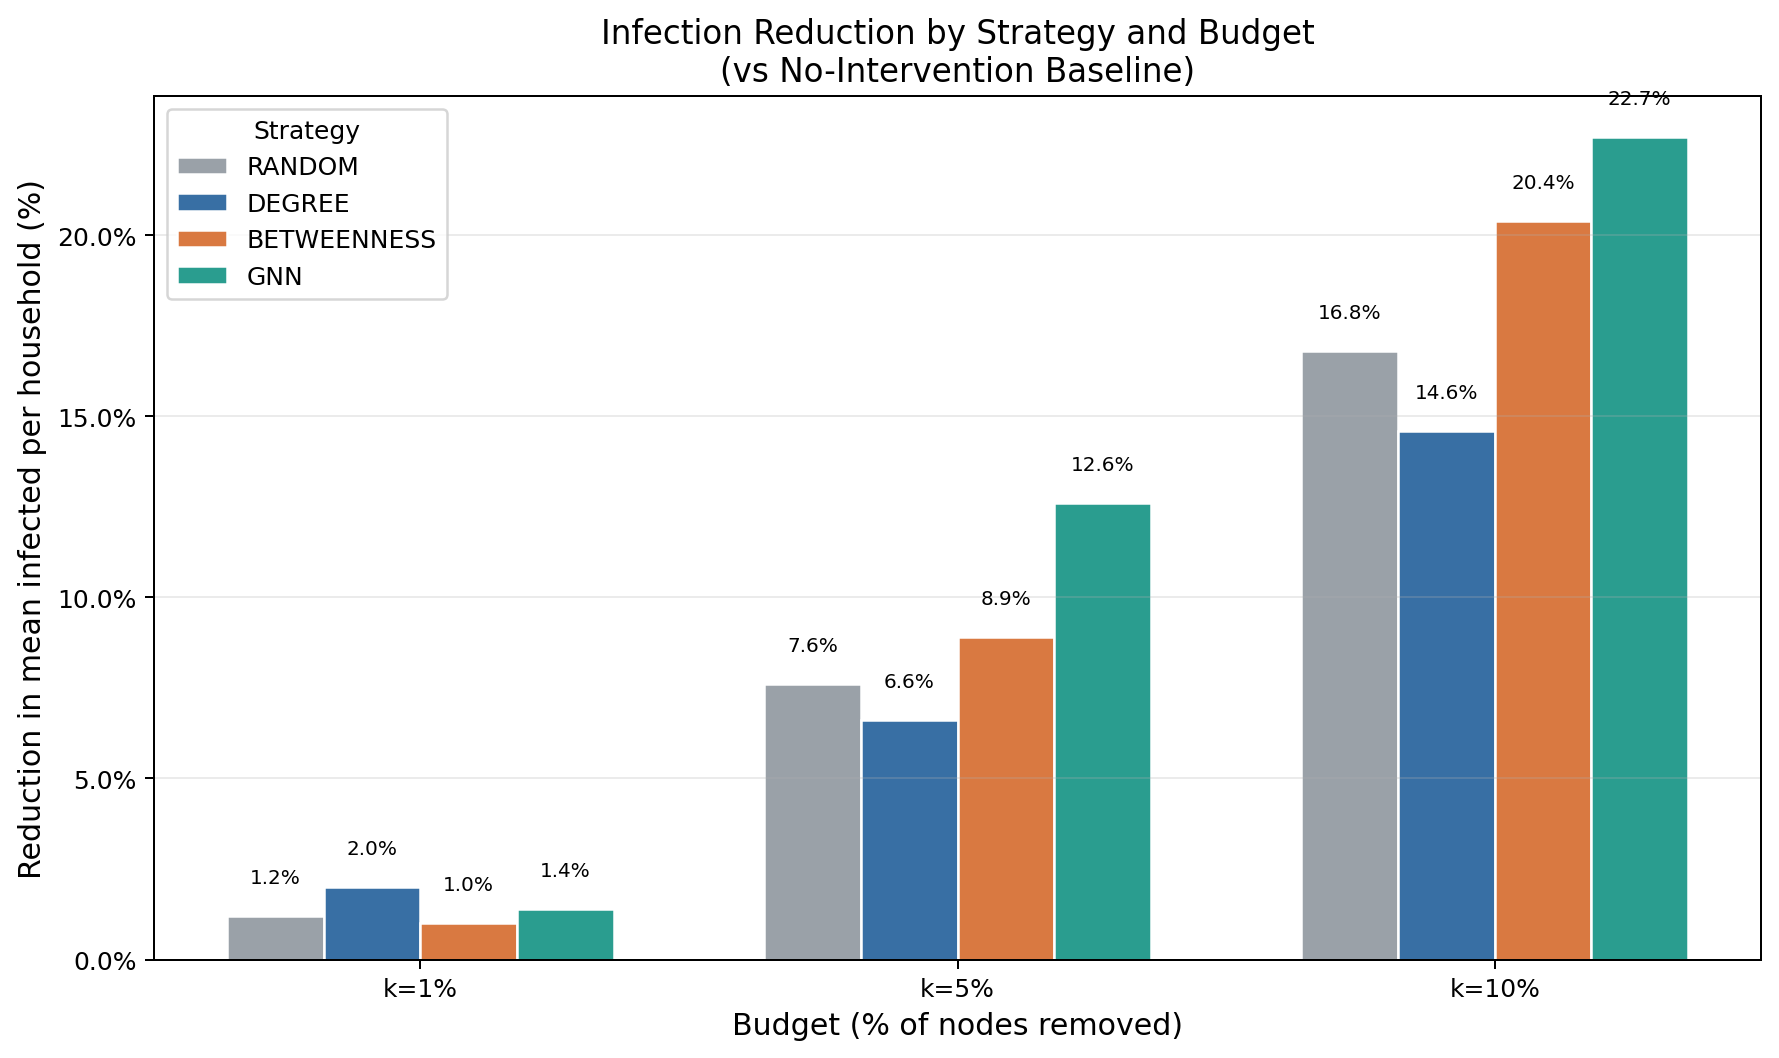
\includegraphics[width=\textwidth]{chart_reduction_by_strategy.png}
  \caption{SIR reduction by strategy.}
\end{subfigure}
\caption{Budget-dependent intervention performance. Source artifacts: \texttt{visualizations/chart\_heatmap.png} and \texttt{visualizations/chart\_reduction\_by\_strategy.png}.}
\label{fig:intervention-performance}
\end{figure}

\section{Discussion}

The results support a budget-sensitive interpretation of intervention strategy. When only three nodes can be selected, direct contact coverage is decisive, and Degree Centrality is a transparent and competitive heuristic. When the budget increases to 17 or 34 nodes, GraphSAGE benefits from combining structural, exposure, and metadata features, leading to larger counterfactual prevention and SIR reductions.

Betweenness is weaker in this dataset because the graph is composed of disconnected household components. Bridge-like nodes are often important in networks with cross-community paths, but SASHTS contains no observed cross-household edges. This limits the value of global bridge-based intervention and shifts emphasis toward direct household exposure and local risk ranking.

These findings should be interpreted as evidence from a single household contact network. They do not establish universal superiority of graph learning for epidemic intervention. Instead, they suggest a conditional rule: use simple centrality when budget is extremely scarce and explainability is critical; use multi-feature graph learning when the intervention set is large enough for learned ranking to exploit richer risk signals.

\section{Limitations}

This study has several limitations. First, the dataset contains 340 individuals in 88 household components, which limits external validity for schools, workplaces, hospitals, or city-scale contact networks. Second, Klerksdorp records lack real timestamps, so the present analysis is static rather than fully temporal. Third, the Weighted GraphSAGE model is a proxy and not a full reproduction of DeepTrace. Fourth, the node-level split and globally normalized features require leakage audit before submission. Fifth, the SIR model uses simplifying assumptions and has not yet undergone sensitivity analysis. Sixth, the intervention analysis assumes selected nodes can be fully removed or intervened on, which is not a validated public-health deployment model.

\section{Conclusion}

\costtrace\ demonstrates a reproducible graph-analysis workflow for budget-constrained intervention ranking in a household epidemic contact network. The results show that Degree Centrality is strong under an extremely low budget, while a GraphSAGE-based risk score performs better at moderate budgets under both counterfactual and SIR evaluation. The manuscript should be considered a proof of concept until additional leakage controls, sensitivity analyses, stronger baselines, and external datasets are added.

\section*{Ethics Statement}

\TODO{Confirm exact ethics wording with the corresponding author and the dataset access conditions. Current repository evidence describes SASHTS as an academic research dataset. This study performs secondary computational analysis and does not implement real medical intervention.}

\section*{Data Availability}

\TODO{Confirm whether raw SASHTS files may be redistributed. If not, replace with a statement that code and derived non-sensitive artifacts are available, while raw data must be obtained from the original data provider subject to its license/access conditions.}

\section*{Code Availability}

The analysis code is organized under \texttt{src/costtrace/}, with the main entry point \texttt{main.py}. Key result artifacts are stored under \texttt{results/}. \TODO{Insert final repository URL and commit hash for submission.}

\section*{Funding}

\TODO{Add funding statement or state that no external funding was received.}

\section*{Conflicts of Interest}

\TODO{Add conflict-of-interest statement for all authors.}

\section*{Author Contributions}

\TODO{Add author contribution taxonomy after final author order is confirmed.}

\section*{AI/Tool Use Disclosure}

\TODO{Add disclosure if required by the target journal.}

\begin{thebibliography}{99}

\bibitem{hamilton2017graphsage}
Hamilton WL, Ying R, Leskovec J.
Inductive representation learning on large graphs.
In: Advances in Neural Information Processing Systems. 2017;30.

\bibitem{blondel2008louvain}
Blondel VD, Guillaume JL, Lambiotte R, Lefebvre E.
Fast unfolding of communities in large networks.
Journal of Statistical Mechanics: Theory and Experiment. 2008;2008(10):P10008.

\bibitem{keeling2005networks}
Keeling MJ, Eames KTD.
Networks and epidemic models.
Journal of the Royal Society Interface. 2005;2(4):295--307.

\bibitem{kiss2017epidemics}
Kiss IZ, Miller JC, Simon PL.
Mathematics of Epidemics on Networks: From Exact to Approximate Models.
Springer; 2017.

\bibitem{freeman1977centrality}
Freeman LC.
A set of measures of centrality based on betweenness.
Sociometry. 1977;40(1):35--41.

\bibitem{newman2006modularity}
Newman MEJ.
Modularity and community structure in networks.
Proceedings of the National Academy of Sciences. 2006;103(23):8577--8582.

\bibitem{kermack1927sir}
Kermack WO, McKendrick AG.
A contribution to the mathematical theory of epidemics.
Proceedings of the Royal Society of London. Series A. 1927;115(772):700--721.

\bibitem{tan2025deeptrace}
Tan CW, Yu PD, Chen S, Poor HV.
DeepTrace: Learning to optimize contact tracing in epidemic networks with graph neural networks.
arXiv preprint. \TODO{Verify final publication metadata before submission.}

\bibitem{sashts}
Kleynhans J, et al.
SARS-CoV-2 household transmission study (SASHTS): physical proximity contact sensor data and epidemiological outcomes.
\TODO{Verify official dataset citation, DOI/URL, and access statement before submission.}

\end{thebibliography}

\end{document}
